\section{Signals}

\subsection{Sinusoids}

\begin{frame}[plain]{Continuous-Time Sinusoidal Signal}
    \begin{equation}\label{eq:cosine}
        x(t) = A\cos(\omega_0 t + \phi).
    \end{equation}


    \begin{figure}
        \centering
        \pgfplotsset{compat=1.12}
\pgfplotsset{every tick label/.append style={font=\scriptsize}}
  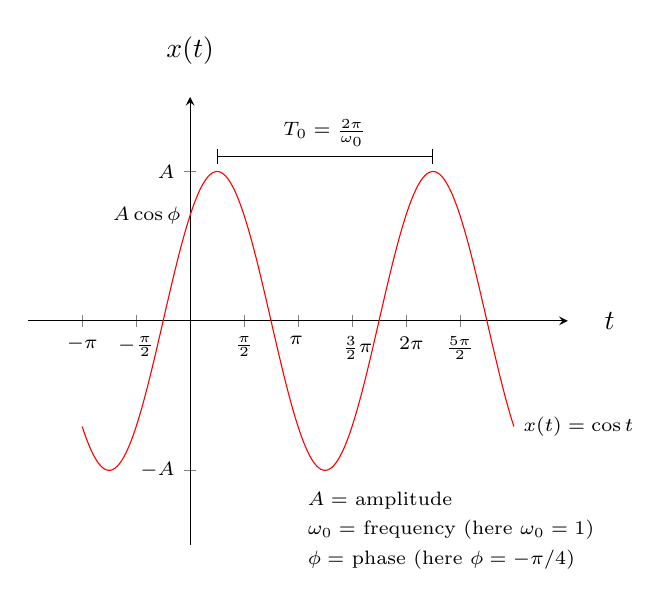
\begin{tikzpicture}
  \def\omwga0{2*pi}
  \def\phase{-45}
    \begin{axis}[
     clip=false,
     xmin=-1.5*pi,xmax=3.5*pi,
     xlabel= $t$,
     ylabel=$ x(t)$,
     ymin=-1.5,ymax=1.5,
     axis lines=middle,
     %axis x line=middle,
     %axis y line=left,
%     axis x line=middle,
     xtick={-3.14, -1.57, 0,1.57,3.14,4.71,6.28, 7.85},
     xticklabels={$-\pi$, $-\frac{\pi}{2}$, $0$, $\frac{\pi}{2}$,$\pi\,$,$\,\,\,\frac{3}{2}\pi$,$\,\,\,2\pi$, $\frac{5\pi}{2}$},
     ytick={-1, 1},
     yticklabels={$\small  -A$, $\small  A$},
     %xticklabel style={anchor=north west}
     every axis x label/.style={
    at={(ticklabel* cs:1.05)},
    anchor=west,
},
every axis y label/.style={
    at={(ticklabel* cs:1.05)},
    anchor=south,
},
     ]
      \addplot[domain=-pi:3*pi,samples=200,red]{cos(deg(x) + \phase)}
                                node[right,pos=1,font=\footnotesize, black]{\scriptsize $x(t)=\cos t$};


       \draw[|-|] (axis cs: pi/4,1.1) -- (axis cs: 2*pi +pi/4,1.1) node[midway, above] {\scriptsize $T_0=\frac{2\pi}{\omega_0}$};
       \node at (axis cs:0, .707) [anchor=east] {\scriptsize $A\cos\phi$  };

       \node at (axis cs:pi, -1.2) [anchor=west] {\scriptsize $A =$ amplitude };
       \node at (axis cs:pi, -1.4) [anchor=west] {\scriptsize $\omega_0 =$ frequency (here $\omega_0 =1$) };
       \node at (axis cs:pi, -1.6) [anchor=west] {\scriptsize $\phi =$ phase (here $\phi =-\pi/4$) };
    \end{axis}


  \end{tikzpicture} 
        \caption{Continuous-time sinusoidal signal.}\label{fi:cosine}
    \end{figure}
\end{frame}

\begin{frame}[plain]{Periodicity of a Sinusoidal}
    Sinusoidal signal is \alert{periodic}.\\
    A periodic continuous-time signal $x(t)$ has the property that  there is a positive value $T$ for which
    \begin{equation}\label{eq:period}
        x(t) = x(t+T)
    \end{equation}
    for all values of $t$. Under an appropriate time-shift the signal repeats itself. In this case we say that $x(t)$ is periodic with period $T$.\\
    \alert{Fundamental period $T_0$} = smallest positive value of $T$ for which \ref{eq:period} holds.\\
    A signal that is not periodic is referred to as aperiodic. \\
    E.g.: Consider $A\cos(\omega_0t + \phi)$\\
    \begin{equation*}
        \begin{split}
            A\cos(\omega_0t + \phi) &= A\cos(\omega_0(t + T) + \phi)\quad \text{ here } \omega_0T = 2\pi m \quad \text{an integer multiple of } 2\pi\\
                                    &= A\cos(\omega_0t + \phi)\\
        \end{split}
    \end{equation*}
    $T = \frac{2\pi m}{\omega_0} \Rightarrow $ fundamental period $T_0 = \frac{2\pi}{\omega_0}$.

\end{frame}


\begin{frame}[plain]{Phase of a Sinusoidal}
    A time-shift in a CT sinusoid is equivalent to a phase shift.\\
    E.g.: Show that a time-shift of a sinusoid is equal to a phase shift.
    \mode<beamer>
    {
        \begin{equation*}
            A\cos[\omega_0(t + t_0)] = A\cos(\omega_0t + \omega_0t_0) = A\cos(\omega_0t + \Delta\phi),\quad \Delta\phi \text{ is a change in phase}.
        \end{equation*}

        \begin{equation*}
            A\cos[\omega_0(t + t_0) + \phi] = A\cos(\omega_0t + \omega_0t_0 + \phi) = A\cos(\omega_0(t + t_1)),\quad t_1 = t_0 + \phi/\omega_0.
        \end{equation*}
    }
\end{frame}

\begin{frame}[t]
\frametitle{Even and Odd Signals}
    A signal $x(t)$ or $x[n]$ is referred to as an \emph{even} signal if it is identical to its time-reversed counterpart, i.e., with its reflection about the origin:
    \begin{align*}
        x(-t) &= x(t)\\
        x[-n] &= x[n]
    \end{align*}
    A is referred to as an \emph{odd} if
    \begin{align*}
        x(-t) &= -x(t)\\
        x[-n] &= -x[n]
    \end{align*}   
    An odd signal must be ) at $t=0$ or $n=0$. 

    A signal can be broken into a sum of two signals, one of which is even adn one fo which is odd.
    Even part of $x(t)$ is
    \begin{equation*}
        \mathfrak{Ev}\{x(t)\} = \frac{1}{2}[x(t)+x(-t)]
    \end{equation*}
    Odd part of $x(t)$ is
    \begin{equation*}
        \mathfrak{Od}\{x(t)\} = \frac{1}{2}[x(t)-x(-t)]
    \end{equation*}   
\end{frame}


\begin{frame}[plain]\frametitle{Phase of a Sinusoidal: $\phi = 0$}
    \mode<beamer>
    {
        \begin{columns}[t]
            \column{0.5\textwidth}
            {
                \centering
                \pgfplotsset{compat=1.12}
\pgfplotsset{every tick label/.append style={font=\scriptsize}}
  \begin{tikzpicture}
  \def\omwga0{2*pi}
  \def\phase{0}
    \begin{axis}[
     clip=false,
     xmin=-1.5*pi,xmax=3.5*pi,
     xlabel= $t$,
     ylabel={$ x(t) = A\cos(\omega_0 t)$},
     ymin=-1.5,ymax=1.5,
     axis lines=middle,
     %axis x line=middle,
     %axis y line=left,
%     axis x line=middle,
     xtick={6.28},
     xticklabels={$T_0$},
     ytick={-1, 1},
     yticklabels={$\small  -A$, $\small  A$},
     %xticklabel style={anchor=north west}
     every axis x label/.style={
    at={(ticklabel* cs:1.05)},
    anchor=west,
},
every axis y label/.style={
    at={(ticklabel* cs:1.05)},
    anchor=south,
},
     ]
      \addplot[domain=-pi:3*pi,samples=200,red]{cos(deg(x) + \phase)};


       \draw[|-|] (axis cs: 0,1.1) -- (axis cs: 2*pi,1.1) node[midway, above] {\scriptsize $T_0=\frac{2\pi}{\omega_0}$};
       \draw[dashed] (axis cs:2*pi, 0) -- (axis cs:2*pi, 1);
       %\node at (axis cs:0, .707) [anchor=east] {\scriptsize $A\cos\phi$  };

      % \node at (axis cs:pi, -1.2) [anchor=west] {\scriptsize $A =$ amplitude };
       %\node at (axis cs:pi, -1.4) [anchor=west] {\scriptsize $\omega_0 =$ frequency (here $\omega_0 =1$) };
       %\node at (axis cs:pi, -1.6) [anchor=west] {\scriptsize $\phi =$ phase (here $\phi =-\pi/4$) };
    \end{axis}


  \end{tikzpicture} 
            }
            \column{0.4\textwidth}
            {
                \noindent This signal is \alert{even}. If we mirror an even signal about the time origin, it would look exactly the same.\\[12pt]
                Periodic: $x(t) = x(t+ T)$.\\
                Even: $x(t) = x(-t)$.
            }
        \end{columns}
    }
\end{frame}

\begin{frame}[plain]{Phase of a Sinusoidal: $\phi = -\pi/2$}
    \mode<beamer>
    {
        \begin{columns}[t]
            \column{0.5\textwidth}
            {
                \centering
                \pgfplotsset{compat=1.12}
\pgfplotsset{every tick label/.append style={font=\scriptsize}}
  \begin{tikzpicture}
  \def\omwga0{2*pi}
  \def\phase{-90}
    \begin{axis}[
     clip=false,
     xmin=-1.5*pi,xmax=3.5*pi,
     xlabel= $t$,
     ylabel={$ x(t) = A\cos(\omega_0 t - \pi/2)$},
     ymin=-1.5,ymax=1.5,
     axis lines=middle,
     %axis x line=middle,
     %axis y line=left,
%     axis x line=middle,
     xtick={6.28},
     xticklabels={$T_0$},
     ytick={-1, 1},
     yticklabels={$\small  -A$, $\small  A$},
     %xticklabel style={anchor=north west}
        x label style={at={(current axis.right of origin)},anchor=west},
        y label style={at={(current axis.above origin)}, anchor=south},
     ]
      \addplot[domain=-pi:3*pi,samples=200,red]{cos(deg(x) + \phase)};


       \draw[|-|] (axis cs: pi/2,1.1) -- (axis cs: 2.5*pi,1.1) node[midway, above] {\scriptsize $T_0=\frac{2\pi}{\omega_0}$};
       %\draw[dashed] (axis cs:2*pi, 0) -- (axis cs:2*pi, 1);
       %\node at (axis cs:0, .707) [anchor=east] {\scriptsize $A\cos\phi$  };

      % \node at (axis cs:pi, -1.2) [anchor=west] {\scriptsize $A =$ amplitude };
       %\node at (axis cs:pi, -1.4) [anchor=west] {\scriptsize $\omega_0 =$ frequency (here $\omega_0 =1$) };
       %\node at (axis cs:pi, -1.6) [anchor=west] {\scriptsize $\phi =$ phase (here $\phi =-\pi/4$) };
    \end{axis}


  \end{tikzpicture} 
            }
            \column{0.4\textwidth}
            {
                \noindent This signal is \alert{odd}. If we flip an odd signal about the time origin, we also multiply it by a ($-$) sign to get the original signal.\\[12pt]
                Periodic: $x(t) = x(t+ T)$.\\
                Odd: $x(t) = -x(-t)$.
            }
        \end{columns}
    }
\end{frame}

\subsection{Discrete-Time Sinusoidal Signal}

\begin{frame}[plain]{$x[n] = A\cos(\omega_0n+\phi)$ with $\phi = 0$}
    \mode<beamer>
    {
        \begin{columns}[t]
            \column{0.5\textwidth}
            {
                \centering
                
\begin{tikzpicture}
\begin{axis}
[%%%%%%%%%%%%%%%%%%%%%%%%%%%%%%%%%%%
    scale=1,
    axis x line=middle,
    axis y line=middle,
    every axis plot post/.style={mark options={fill=black, mark size=1}},
    xmin=-36,
    xmax=36,
    %xtick={1, 2, 3, 4},
    %xticklabels={1, 2, 3, 4},
    %extra x ticks={-4, -3, -2, -1},
   % extra x tick labels={-4, -3, -2, -1},
   % extra x tick style={ xticklabel style={yshift=0.5ex, anchor=south} },
    xlabel={$n$},
    ylabel={$x[n] = A\cos(\omega_0n)$},
    %ytick={-2,-1, 0, 1, 2},
    xticklabels=\empty,
    ymin=-1.5,
    ymax=1.5,
    x label style={at={(current axis.right of origin)},anchor=west},
    y label style={at={(current axis.above origin)}, anchor=south},
]
\addplot+[ycomb,blue, mark options={black, mark size=1}] table [x={n}, y={xn}] {b_signals/figures/dt_sinusoid_n_16.dat};
\end{axis}
\end{tikzpicture} 
            }
            \column{0.4\textwidth}
            {
                \noindent The independent variable is an integer.\\
                The sequence takes values only at integer values of the argument.\\
                This signal is \alert{even}. \\[12pt]
                Even: $x[n] = x[-n]$.\\
                Periodic: $x[n] = x[n+N]$. Here, $N=16$\\
                $\omega_0 = \frac{2\pi}{N} = \frac{\pi}{8}$.


            }
        \end{columns}
    }
\end{frame}


\begin{frame}[plain]{$x[n] = A\cos(\omega_0n+\phi)$ with $\phi = -\pi/2$}
    \mode<beamer>
    {
        \begin{columns}[t]
            \column{0.5\textwidth}
            {
                \centering
                
\begin{tikzpicture}
\begin{axis}
[%%%%%%%%%%%%%%%%%%%%%%%%%%%%%%%%%%%
    scale=1,
    axis x line=middle,
    axis y line=middle,
    every axis x label={at={(current axis.right of origin)},anchor=north west},
    every axis y label={at={(current axis.above origin)},anchor= north west},
    every axis plot post/.style={mark options={fill=black, mark size=1}},
    xmin=-36,
    xmax=36,
    %xtick={1, 2, 3, 4},
    %xticklabels={1, 2, 3, 4},
    %extra x ticks={-4, -3, -2, -1},
   % extra x tick labels={-4, -3, -2, -1},
   % extra x tick style={ xticklabel style={yshift=0.5ex, anchor=south} },
    xlabel={$n$},
    ylabel={$x[n] = A\cos(\omega_0n - \pi/2)$},
    %ytick={-2,-1, 0, 1, 2},
    xticklabels=\empty,
    ymin=-1.5,
    ymax=1.5,
         every axis x label/.style={at={(ticklabel* cs:1)}, anchor=west,},
         every axis y label/.style={at={(ticklabel* cs:1.05)}, anchor=south,},
]
\addplot+[ycomb,blue, mark options={black, mark size=1}] table [x={n}, y={xn}] {b_signals/figures/dt_sinusoid_n_16_phi_90.dat};
\end{axis}
\end{tikzpicture} 
            }
            \column{0.4\textwidth}
            {
                \noindent The independent variable is an integer.\\
                The sequence takes values only at inter values of he argument.\\
                This signal is \alert{odd}. \\[12pt]
                Odd: $x[n] = -x[-n]$.\\
                Periodic: $x[n] = x[n+N]$. Here, $N=16$\\
                $\omega_0 = \frac{2\pi}{N} = \frac{\pi}{8}$.
                $\phi= -\pi/2$, $x[n] = A\cos(\omega_0n+\phi) = A\cos(\omega_0(n+n_0))$. $n_0$ must be an integer.\\
                $n_0 = \frac{\phi}{\omega_0} = \frac{\pi/2}{\pi/8} = 4$.


            }
        \end{columns}
    }
\end{frame}


\begin{frame}{Phase Change and Time Shift in DT}
    \begin{block}{Q}
        Does a phase change always correspond to a time shift in discrete-time signals?
    \end{block}
    \pause
    \mode<beamer>
    {
        Answer: No.\\
        \begin{align*}
          A\cos[\omega_0n+ \phi)] &=  A\cos[\omega_0(n+n_0)]\\
          \omega_0n + \omega_0n_0 &= \omega_0n + \phi \\
          \omega_0n_0 &= \phi\quad n_0 \text{ is an integer}.
        \end{align*}

        \begin{itemize}
          \item Depending on $\phi$ and $\omega_0$, $n_0$ many not come out to be an \alert{integer}.
          \item In discrete time, the amount of time shift must be an integer.
        \end{itemize}
    }
\end{frame}

\begin{frame}{Periodicity of a DT Signal}
    All continuous-time sinusoids are  periodic. However, discrete-time sinusoids are not necessarily so.
    \begin{equation}
        x[n] = x[n+N], \quad \text{smallest integer $N$ is the fundamental period}.
    \end{equation}
    \mode<beamer>
    {
        \begin{equation*}
            A\cos[\omega_0(n+N) + \phi] = A\cos[\omega_0n+ \omega_0N + \phi]
        \end{equation*}
        $ \omega_0N$ must be an integer multiple of $2\pi$.\\
        Periodic $\Rightarrow$ $\omega_0N = 2\pi m$
        \begin{equation}\label{eq:dt_period}
            N = \frac{2\pi m}{\omega_0}
        \end{equation}
        $N$ and $m$ must be integers.\\
        Smallest $N$, if any, is the fundamental period.\\
        $N$ may not be an integer. In this case, the signal is not periodic.
    }
\end{frame}

\subsection{Exponentials}

\begin{frame}[plain]{CT Real Exponentials}
    \begin{equation*}
        \begin{split}
            x(t) &= Ce^{a(t+t_0)}, \quad C \text{ and } a \text{ are real numbers}\\
            &=   Ce^{at_0}e^{at}.\\
        \end{split}
    \end{equation*}
    \mode<beamer>
    {
        {
            \centering
            \pgfplotsset{compat=1.12}
\pgfplotsset{every tick label/.append style={font=\scriptsize}}
  \begin{tikzpicture}

  \def\a{0.8}
  \def\C{0.2}
    \begin{axis}[
     clip=false,
     xmin=-3,xmax=3,
     xlabel= $t$,
     ylabel=$ x(t)$,
     ymin=-0.2,ymax=1.5,
     axis lines=middle,
     %axis x line=middle,
     %axis y line=left,
%     axis x line=middle,
     xtick=\empty,
     xticklabels={$-\pi$, $-\frac{\pi}{2}$, $0$, $\frac{\pi}{2}$,$\pi\,$,$\,\,\,\frac{3}{2}\pi$,$\,\,\,2\pi$, $\frac{5\pi}{2}$},
     ytick=\empty,
     yticklabels={$\small  -A$, $\small  A$},
     %xticklabel style={anchor=north west}
     every axis x label/.style={
    at={(ticklabel* cs:1)},
    anchor=west,
},
every axis y label/.style={
    at={(ticklabel* cs:1)},
    anchor=south,
},
     ]
      \addplot[domain=-2:2,samples=200,red]{\C*exp(\a*x)}
                                node[right,pos=1,font=\footnotesize, black]{\scriptsize $x(t)=Ce^{at}$};

	\node at (axis cs:1, 1) [anchor=east] {\scriptsize $a > 0$  };

    \end{axis}
    
    \begin{scope}[xshift=8cm]
      \def\a{-0.8}
  \def\C{0.2}
    \begin{axis}[
     clip=false,
     xmin=-3,xmax=3,
     xlabel= $t$,
     ylabel=$ x(t)$,
     ymin=-0.2,ymax=1.5,
     axis lines=middle,
     %axis x line=middle,
     %axis y line=left,
%     axis x line=middle,
     xtick=\empty,
     xticklabels={$-\pi$, $-\frac{\pi}{2}$, $0$, $\frac{\pi}{2}$,$\pi\,$,$\,\,\,\frac{3}{2}\pi$,$\,\,\,2\pi$, $\frac{5\pi}{2}$},
     ytick=\empty,
     yticklabels={$\small  -A$, $\small  A$},
     %xticklabel style={anchor=north west}
     every axis x label/.style={
    at={(ticklabel* cs:1)},
    anchor=west,
},
every axis y label/.style={
    at={(ticklabel* cs:1)},
    anchor=south,
},
     ]
      \addplot[domain=-2:2,samples=200,red]{\C*exp(\a*x)}
                                node[right,pos=0,font=\footnotesize, black]{\scriptsize $x(t)=Ce^{at}$};

	\node at (axis cs:1, 1) [anchor=east] {\scriptsize $a < 0$  };

    \end{axis}
\end{scope}


  \end{tikzpicture} 
        }
    }
\end{frame}

\begin{frame}[plain]{DT Real Exponentials}
    \begin{equation*}
        x[n] = Ce^{\beta n} = C\alpha^n, \quad C \text{ and } \alpha \text{ are real numbers}
    \end{equation*}
\end{frame}

\begin{frame}[plain]
    \mode<beamer>
    {
        {
            \centering
            
\begin{tikzpicture}

\begin{scope}
\begin{axis}
[
    scale=1,
    axis x line=middle,
    axis y line=middle,
    every axis x label={at={(current axis.right of origin)},anchor=north west},
    every axis y label={at={(current axis.above origin)},anchor= north west},
    every axis plot post/.style={mark options={fill=black, mark size=1}},
    xmin=-25,
    xmax=25,
    xlabel={$n$},
    ylabel={$x[n] = C\alpha^n, \quad \alpha = 0.92$},
    ymin=-5.5,
    ymax=5.5,
         every axis x label/.style={at={(ticklabel* cs:1)}, anchor=west,},
         every axis y label/.style={at={(ticklabel* cs:1.05)}, anchor=south,},
]
\addplot+[ycomb,blue, mark options={black, mark size=1}] table [x={n}, y={xn}] {b_signals/figures/dt_exp_alpha_pos_less_than_one.dat};
\node at (axis cs: -22, -2) {$\alpha > 0, | \alpha | < 1$};
\end{axis}
\end{scope}


\begin{scope}[xshift=8cm]
\begin{axis}
[
    scale=1,
    axis x line=middle,
    axis y line=middle,
    every axis x label={at={(current axis.right of origin)},anchor=north west},
    every axis y label={at={(current axis.above origin)},anchor= north west},
    every axis plot post/.style={mark options={fill=black, mark size=1}},
    xmin=-25,
    xmax=25,
    xlabel={$n$},
    ylabel={$x[n] = C\alpha^n, \quad \alpha = 1.08$},
    ymin=-5.5,
    ymax=5.5,
         every axis x label/.style={at={(ticklabel* cs:1)}, anchor=west,},
         every axis y label/.style={at={(ticklabel* cs:1.05)}, anchor=south,},
]
\addplot+[ycomb,blue, mark options={black, mark size=1}] table [x={n}, y={xn}] {b_signals/figures/dt_exp_alpha_pos_greater_than_one.dat};
\node at (axis cs: -22, -2) {$\alpha > 0, | \alpha | > 1$};
\end{axis}
\end{scope}



\end{tikzpicture} 
        }
    }
\end{frame}

\begin{frame}[plain]
    \mode<beamer>
    {
        {
            \centering
            
\begin{tikzpicture}
\begin{axis}
[
    scale=1,
    axis x line=middle,
    axis y line=middle,
    x label style={at={(current axis.right of origin)},anchor=west},
    y label style={at={(current axis.above origin)}, anchor=south},
    every axis plot post/.style={mark options={fill=black, mark size=1}},
    xmin=-25,
    xmax=25,
    xlabel={$n$},
    ylabel={$x[n] = C\alpha^n, \quad \alpha = -0.92$},
    ymin=-5.5,
    ymax=5.5,
]
\addplot+[ycomb,blue, mark options={black, mark size=1}] table [x={n}, y={xn}] {b_signals/figures/dt_exp_alpha_neg_less_than_one.dat};
\node at (axis cs: 8, -2) {$\alpha < 0, | \alpha | < 1$};
\end{axis}

\begin{scope}[xshift=8cm]
\begin{axis}
[
    scale=1,
    axis x line=middle,
    axis y line=middle,
    x label style={at={(current axis.right of origin)},anchor=west},
    y label style={at={(current axis.above origin)}, anchor=south},
    every axis plot post/.style={mark options={fill=black, mark size=1}},
    xmin=-25,
    xmax=25,
    xlabel={$n$},
    ylabel={$x[n] = C\alpha^n, \quad \alpha = -1.08$},
    ymin=-5.5,
    ymax=5.5,
]
\addplot+[ycomb,blue, mark options={black, mark size=1}] table [x={n}, y={xn}] {b_signals/figures/dt_exp_alpha_neg_greater_than_one.dat};
\node at (axis cs: -22, -2) {$\alpha < 0, | \alpha | > 1$};
\end{axis}
\end{scope}


\end{tikzpicture} 
        }
    }
\end{frame}


\subsection{CT Complex Exponentials}
\begin{frame}[plain]{CT Complex Exponentials}
    \tikzstyle{na} = [baseline=-.5ex]
    \tikzstyle{every picture}+=[remember picture]
    \begin{align*}
            x(t) &= Ce^{at} \quad C \text{ and } a \text{ are complex numbers}.\\
            C &= |C|e^{j\theta}\\
            a &= r + j\omega_0\\
            x(t) &= |C|e^{j\theta}e^{(r + j\omega_0)t}\\
            &= |C|e^{rt}
            \tikz[baseline]{
            \node[fill=blue!20,anchor=base] (t1)
            {$e^{j(\omega_0t + \theta)}$};
            }
            \\
            &=
            \tikz[baseline]{
            \node[fill=red!20,anchor=base] (t2)
            {
                $|C|e^{rt}$
            };
            }
            \left[\cos(\omega_0t + \theta)\right. +
            \tikz[baseline]{
            \node[fill=green!20,anchor=base] (t3)
            {
                $j$
            };
            }
            \left.\sin(\omega_0t + \theta)\right]\\
    \end{align*}

    \mode<beamer>
    {
        \pause
        \begin{itemize}[<+-| alert@+>]
            \item $e^{j(\omega_0t + \theta)} = \cos(\omega_0t + \theta) + j\sin(\omega_0t + \theta)$
                \tikz[na]\node [coordinate] (n1) {};
            \item Real
                \tikz[na]\node [coordinate] (n2) {};
            \item $90^\circ$ out of phase
                \tikz[na]\node [coordinate] (n3) {};
        \end{itemize}

        % Now it's time to draw some edges between the global nodes. Note that we
        % have to apply the 'overlay' style.
        \begin{tikzpicture}[overlay]
                \path[->]<1-> (n1) edge [bend right] (t1);
                \path[->]<2-> (n2) edge [bend right] (t2);
                \path[->]<3-> (n3) edge [bend right] (t3);
        \end{tikzpicture}
    }
\end{frame}


\begin{frame}[plain]
    \mode<beamer>
    {
        {
            \centering
            \pgfplotsset{compat=1.12}
\pgfplotsset{every tick label/.append style={font=\scriptsize}}
  \begin{tikzpicture}
  \def\omwga0{2*pi}
  \def\phase{-45}
  \def\r{0.4}
    \begin{axis}[
    scale=0.8,
     clip=false,
     xmin=-6,xmax=6,
     xlabel= $t$,
     ylabel={$x(t)=|C|e^{rt}\cos(\omega_0t+\phi)$},
     ymin=-10,ymax=10,
     axis lines=middle,
     %axis x line=middle,
     %axis y line=left,
%     axis x line=middle,
     xtick={-3.14, -1.57, 0,1.57,3.14,4.71,6.28, 7.85},
     %xticklabels={$-\pi$, $-\frac{\pi}{2}$, $0$, $\frac{\pi}{2}$,$\pi\,$,$\,\,\,\frac{3}{2}\pi$,$\,\,\,2\pi$, $\frac{5\pi}{2}$},
     xticklabels=\empty,
     ytick={-1, 1},
     yticklabels=\empty,
     %xticklabel style={anchor=north west}
        x label style={at={(current axis.right of origin)},anchor=west},
        y label style={at={(current axis.above origin)}, anchor=south},
     ]
      \addplot[domain=-5:5,samples=200,red]{exp(\r*x)*cos(2*pi*deg(x))};
      \addplot[domain=-5:5,samples=200,blue, dashed]{exp(\r*x)}
                                node[right,pos=1,font=\footnotesize, black]{\scriptsize $e^{rt}$};
                                      \addplot[domain=-5:5,samples=200,blue, dashed]{-exp(\r*x)}
                                node[right,pos=1,font=\footnotesize, black]{\scriptsize $-e^{rt}$};
       \node at (axis cs:2, 8) [anchor=west] {\scriptsize $r>0$ };
    \end{axis}


    \begin{scope}[xshift=9cm]

  \def\omwga0{2*pi}
  \def\phase{-45}
  \def\r{-0.4}
    \begin{axis}[
    scale=0.8,    
     clip=false,
     xmin=-6,xmax=6,
     xlabel= $t$,
     ylabel={$x(t)=|C|e^{rt}\cos(\omega_0t+\phi)$},
     ymin=-10,ymax=10,
     axis lines=middle,
     %axis x line=middle,
     %axis y line=left,
%     axis x line=middle,
     xtick={-3.14, -1.57, 0,1.57,3.14,4.71,6.28, 7.85},
     %xticklabels={$-\pi$, $-\frac{\pi}{2}$, $0$, $\frac{\pi}{2}$,$\pi\,$,$\,\,\,\frac{3}{2}\pi$,$\,\,\,2\pi$, $\frac{5\pi}{2}$},
     xticklabels=\empty,
     ytick={-1, 1},
     yticklabels=\empty,
     %xticklabel style={anchor=north west}
        x label style={at={(current axis.right of origin)},anchor=west},
        y label style={at={(current axis.above origin)}, anchor=south},
     ]
      \addplot[domain=-5:5,samples=200,red]{exp(\r*x)*cos(2*pi*deg(x))};
      \addplot[domain=-5:5,samples=200,blue, dashed]{exp(\r*x)}
                                node[right,pos=0,font=\footnotesize, black]{\scriptsize $e^{rt}$};
                                      \addplot[domain=-5:5,samples=200,blue, dashed]{-exp(\r*x)}
                                node[right,pos=0,font=\footnotesize, black]{\scriptsize $-e^{rt}$};
       \node at (axis cs:2, 8) [anchor=west] {\scriptsize $r<0$ };
    \end{axis}

	\end{scope}


  \end{tikzpicture} 
        }
    }
\end{frame}



\begin{frame}[plain]{DT Complex Exponentials}
    \begin{align}
        x[n] &= C\alpha^n, \quad C \text{ and } \alpha \text{ are complex numbers.}\\
        C &= |C|e^{j\theta}\\
        \alpha &= |\alpha|e^{j\omega_0}\\
        x[n] &= |C|e^{j\theta}\left(|\alpha|e^{j\omega_0}\right)^n\\
        &= |C||\alpha|^n\cos(\omega_0n + \theta) + j|C||\alpha|^n\sin(\omega_0n + \theta)\\
    \end{align}
    Comments:
    \begin{itemize}
      \item When $|\alpha| = 1$: sinusoidal real and imaginary parts.
      \item $e^{j\omega_0 n}$ may or may not be periodic depending on the value of $\omega_0$.
      \item Sinusoidal, exponential, step, and impulse signal form the cornerstones for signals and systems analysis.
    \end{itemize}
\end{frame}





\begin{frame}[plain]{DT Complex Exponentials Plot}
    \mode<beamer>
    {
        {
            \centering
            
\begin{tikzpicture}
  \def\r{1.12}
\begin{axis}
[
    scale=1,
    axis x line=middle,
    axis y line=middle,
    every axis x label={at={(current axis.right of origin)},anchor=north west},
    every axis y label={at={(current axis.above origin)},anchor= north west},
    every axis plot post/.style={mark options={fill=black, mark size=1}},
    xmin=-25,
    xmax=25,
    xlabel={$n$},
    ylabel={$xn = |C||\alpha|^n\cos(\omega_0n + \theta), \quad |\alpha| = 1.12, \theta = 0$},
    ymin=-7,
    ymax=7,
         every axis x label/.style={at={(ticklabel* cs:1)}, anchor=west,},
         every axis y label/.style={at={(ticklabel* cs:1.05)}, anchor=south,},
]
\addplot+[ycomb,blue, mark options={black, mark size=1}] table [x={n}, y={xn}] {b_signals/figures/dt_complex_exp_alpha_greater_than_one.dat};
      \addplot[domain=-25:25,samples=200,red, dashed]{pow(\r,x)}
                                node[right,pos=1,font=\footnotesize, black]{\scriptsize $e^{rt}$};
                                      \addplot[domain=-25:25,samples=200,red, dashed]{-pow(\r,x)}
                                node[right,pos=1,font=\footnotesize, black]{\scriptsize $-e^{rt}$};
\node at (axis cs: -16, -4) {$| \alpha | >1$};
\end{axis}

\begin{scope}[xshift=8cm]
\def\r{0.92}
\begin{axis}
[
    scale=1,
    axis x line=middle,
    axis y line=middle,
    every axis x label={at={(current axis.right of origin)},anchor=north west},
    every axis y label={at={(current axis.above origin)},anchor= north west},
    every axis plot post/.style={mark options={fill=black, mark size=1}},
    xmin=-25,
    xmax=25,
    xlabel={$n$},
    ylabel={$xn = |C||\alpha|^n\cos(\omega_0n + \theta), \quad |\alpha| = 0.92, \theta = 0$},
    ymin=-7,
    ymax=7,
         every axis x label/.style={at={(ticklabel* cs:1)}, anchor=west,},
         every axis y label/.style={at={(ticklabel* cs:1.05)}, anchor=south,},
]
\addplot+[ycomb,blue, mark options={black, mark size=1}] table [x={n}, y={xn}] {b_signals/figures/dt_complex_exp_alpha_less_than_one.dat};
      \addplot[domain=-25:25,samples=200,red, dashed]{pow(\r,x)}
                                node[right,pos=1,font=\footnotesize, black]{\scriptsize $e^{rt}$};
                                      \addplot[domain=-25:25,samples=200,red, dashed]{-pow(\r,x)}
                                node[right,pos=1,font=\footnotesize, black]{\scriptsize $-e^{rt}$};
\node at (axis cs: -16, -4) {$| \alpha | < 1$};
\end{axis}
\end{scope}


\end{tikzpicture}
%b_signals/figures/ 
        }
    }
\end{frame}




\begin{frame}{Periodicity Properties of Discrete-Time Complex Exponentials $e^{j\omega_0 n}$}
    \begin{itemize}[<+-| alert@+>]
      \item For the CT counterpart  $e^{j\omega_0 t}$,
        \begin{enumerate}
            \item The larger the magnitude of $\omega_0$, the higher is the rate of oscillation in the signal.
            \item $e^{j\omega_0 t}$ is periodic for any value of $\omega_0$.
        \end{enumerate}
      \item In DT, as 
        \begin{equation*}
            e^{j(\omega_0 + 2\pi)n} = e^{j2\pi n}e^{j\omega_0n} = e^{j\omega_0n}
        \end{equation*}
        the exponential at frequency $\omega_0 + 2\pi$ is the same as that at frequency $\omega_0$ .
      \item Although in CT  $e^{j\omega_0 t}$ are all distinct for distinct values of $\omega_0$. In DT, these signals are not distinct, as the signal with frequency $\omega_0$ is identical to the signals with frequencies $\omega_0 + 2\pi$, $\omega_0 + 4\pi$, and so on. Therefore, in considering DT complex exponentials, we need only consider a frequency interval of length $2\pi$ in which to choose $\omega_0$.
      \item In DT, as we increase $\omega_0$ from 0, we obtain signals that oscillate more and more rapidly until we reach $\omega_0 = \pi$. As we continue to increase $\omega_0$, we decrease the rate of oscillation until we reach $\omega_0 = 2\pi$. Note: $e^{j\pi n} = \left(e^{j\pi}\right)^n = (-1)^n$.
    \end{itemize}
    
\end{frame}


\begin{frame}[plain]{Discrete-Time Unit Step  $u[n]$}
    \begin{equation}
        u[n] = \begin{cases}
                 1, & n \geq 0,\\
                 0, & n<0.
               \end{cases}
    \end{equation}
    \mode<beamer>
    {
        {
            \centering
            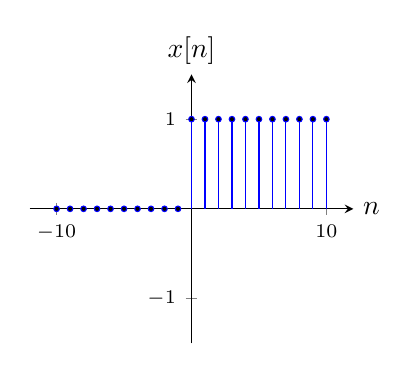
\begin{tikzpicture}
\begin{filecontents}{step.dat}
n	xn
-10	0
-9	0
-8	0
-7	0
-6	0
-5	0
-4	0
-3	0
-2	0
-1	0
0	1
1	1
2	1
3	1
4	1
5	1
6	1
7	1
8	1
9	1
10	1
\end{filecontents}
\begin{axis}
[%%%%%%%%%%%%%%%%%%%%%%%%%%%%%%%%%%%
    scale=0.6,
    axis x line=middle,
    axis y line=middle,
    every axis plot post/.style={mark options={fill=black}},
    xmin=-12,
    xmax=12,
    %xtick={1, 2, 3, 4},
    %xticklabels={1, 2, 3, 4},
    %extra x ticks={-4, -3, -2, -1},
   % extra x tick labels={-4, -3, -2, -1},
   % extra x tick style={ xticklabel style={yshift=0.5ex, anchor=south} },
    xlabel={$n$},
    ylabel={$x[n]$},
    %ytick={-2,-1, 0, 1, 2},
    %xticklabels=\empty,
    ymin=-1.5,
    ymax=1.5,
    x label style={at={(current axis.right of origin)},anchor=west},
    y label style={at={(current axis.above origin)}, anchor=south},
]
\addplot+[ycomb,blue, , mark size=1pt] table [x={n}, y={xn}] {step.dat};
\end{axis}
\end{tikzpicture} 
        }
    }
\end{frame}

\begin{frame}[plain]{Discrete-Time Unit Impulse (Unit Sample) $\delta[n]$}
    \begin{equation}
        \delta[n] = \begin{cases}
                 1, & n = 0,\\
                 0, & n \neq 0.
               \end{cases}
    \end{equation}
    \mode<beamer>
    {
        {
            \centering
            \begin{tikzpicture}[scale=0.6]
\begin{filecontents}{step.dat}
n	xn
-10	0
-9	0
-8	0
-7	0
-6	0
-5	0
-4	0
-3	0
-2	0
-1	0
0	1
1	0
2	0
3	0
4	0
5	0
6	0
7	0
8	0
9	0
10	0
\end{filecontents}
\begin{axis}
[%%%%%%%%%%%%%%%%%%%%%%%%%%%%%%%%%%%
    scale=1,
    axis x line=middle,
    axis y line=middle,
    every axis x label={at={(current axis.right of origin)},anchor=north west},
    every axis y label={at={(current axis.above origin)},anchor= north west},
    every axis plot post/.style={mark options={fill=black}},
    xmin=-12,
    xmax=12,
    %xtick={1, 2, 3, 4},
    %xticklabels={1, 2, 3, 4},
    %extra x ticks={-4, -3, -2, -1},
   % extra x tick labels={-4, -3, -2, -1},
   % extra x tick style={ xticklabel style={yshift=0.5ex, anchor=south} },
    xlabel={$n$},
    ylabel={$x[n]$},
    %ytick={-2,-1, 0, 1, 2},
    %xticklabels=\empty,
    ymin=-1.5,
    ymax=1.5,
     every axis x label/.style={at={(ticklabel* cs:1)}, anchor=west,} ,
     every axis y label/.style={at={(ticklabel* cs:1.05)}, anchor=south,},
]
\addplot+[ycomb,blue] table [x={n}, y={xn}] {step.dat};
\end{axis}
\end{tikzpicture}
        }
    }
\end{frame}


\subsection{Step and Impulse Functions}
\begin{frame}[plain]{DT Step and Impulse}
    Unit impulse is the first backward difference of the unit step sequence.
    \begin{equation}
        \delta[n] = u[n] - u[n-1].
    \end{equation}
    \mode<handout>
    {
        \vspace{1in}
    }

    \mode<beamer>
    {
        {
            \centering
            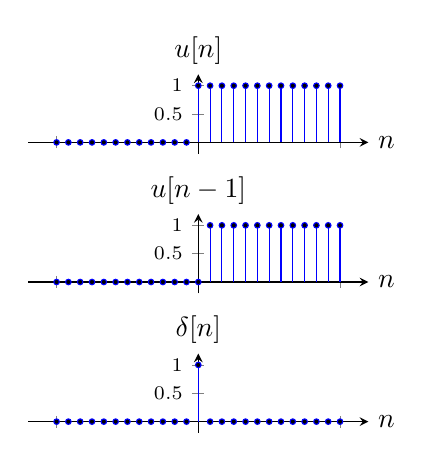
\begin{tikzpicture}[
    declare function={
    unitstep(\x)= (\x>-0.1)*(1);
    impulse(\x,\nn)  = and((\nn-0.5) < \x, \x < \nn)*1;
    unitstepd(\x,\nn)= ((\nn-1)<\x)*(1);
  }
]
\begin{axis}
	[
		name=un,
	    scale=0.6,
	    axis x line=middle,
	    axis y line=middle,
	    every axis plot post/.style={mark options={fill=black}},
	    xmin=-12,
	    xmax=12,
	    xlabel={$n$},
	    ylabel={$u[n]$},
	    xticklabel=\empty,
	    y=1.2cm,
	    x=0.3cm,
	    ymin=-0.2,
	    ymax=1.2,
	    clip=false,
        x label style={at={(current axis.right of origin)},anchor=west},
        y label style={at={(current axis.above origin)}, anchor=south},
	]
	\addplot+[ycomb,domain=-10:10, blue, mark size=1pt ] {unitstep(x)};
\end{axis}

\pause

%\begin{scope}
	\begin{axis}
	[
		name=unminus1,
		at=(un.below south), anchor=above north,
	    scale=0.6,
	    axis x line=middle,
	    axis y line=middle,
	    every axis plot post/.style={mark options={fill=black}},
	    xmin=-12,
	    xmax=12,
	    xlabel={$n$},
	    ylabel={$u[n-1]$},
	    xticklabel=\empty,
	    y=1.2cm,
	    x=0.3cm,
	    ymin=-0.2,
	    ymax=1.2,
	    clip=false,
        x label style={at={(current axis.right of origin)},anchor=west},
        y label style={at={(current axis.above origin)}, anchor=south},
	]
	\addplot+[ycomb,domain=-10:10, blue, mark size=1pt] {unitstepd(x,1)};
	\end{axis}
%\end{scope}
%
\pause
%
%\begin{scope}[yshift=-5cm]
	\begin{axis}
	[
		name=deltanminus2,
		at=(unminus1.below south), anchor=above north,	
	    scale=0.6,
	    axis x line=middle,
	    axis y line=middle,
	    every axis plot post/.style={mark options={fill=black}},
	    xmin=-12,
	    xmax=12,
	    xlabel={$n$},
	    ylabel={$\delta[n]$},
	    xticklabel=\empty,
	    y=1.2cm,
	    x=0.3cm,
	    ymin=-0.2,
	    ymax=1.2,
	    clip=false,
        x label style={at={(current axis.right of origin)},anchor=west},
        y label style={at={(current axis.above origin)}, anchor=south},
	]
	\addplot+[ycomb,domain=-10:10, blue, mark size=1pt] {impulse(x, 0)};
	\end{axis}
\end{tikzpicture} 
        }
    }
\end{frame}

\begin{frame}[plain]{DT Step and Impulse}
    The unit step sequence is the running sum of the unit impulse.
    \begin{equation}
        u[n] = \sum_{m=-\infty}^{n}\delta[m].
    \end{equation}
    \mode<handout>
    {
        \vspace{1in}
    }
    \pause
    \mode<beamer>
    {
        {
            \centering
            \begin{tikzpicture}[scale=0.6,
  declare function={
    unitstep(\x)= (\x>-0.1)*(1);
  },
    declare function={
    unitstepdelayed(\x)= (\x>0.1)*(1);
  },
    declare function={
    impulse(\x)= and(\x>-0.1, \x<0.1)*(1);
  }
]
\begin{axis}
[
    scale=1,
    axis x line=middle,
    axis y line=middle,
    every axis plot post/.style={mark options={fill=black}},
    xmin=-12,
    xmax=12,
    xlabel={$m$},
    ylabel={$$},
    y=1.2cm,
    x=0.3cm,
    ymin=-0.2,
    ymax=1.2,
    clip=false,
        x label style={at={(current axis.right of origin)},anchor=west},
        y label style={at={(current axis.above origin)}, anchor=south},
]
\draw[draw=none, pattern=north west lines, pattern color=red!80!blue!30] (axis cs:-12, 1.2) rectangle (axis cs:-3, 0);
\addplot+[ycomb,domain=-10:10, blue] {impulse(x)};
\draw[red, dashed, thick] (axis cs:-12, 1.2) -| (axis cs:-3, 0) node [anchor=north, yshift=-3pt] {$n$};
\end{axis}

\pause

\begin{scope}[yshift=-3cm]
	\begin{axis}
[
    scale=1,
    axis x line=middle,
    axis y line=middle,
    every axis plot post/.style={mark options={fill=black}},
    xmin=-12,
    xmax=12,
    xlabel={$m$},
    ylabel={$$},
    y=1.2cm,
    x=0.3cm,
    ymin=-0.2,
    ymax=1.2,
    clip=false,
        x label style={at={(current axis.right of origin)},anchor=west},
        y label style={at={(current axis.above origin)}, anchor=south},
]
%\addplot+[ycomb,blue] table [x={n}, y={xn}] {step.dat};
\draw[draw=none, pattern=north west lines, pattern color=red!80!blue!30] (axis cs:-12, 1.2) rectangle (axis cs:3, 0);
\addplot+[ycomb,domain=-10:10, blue] {impulse(x)};
\draw[red, dashed, thick] (axis cs:-12, 1.2) -| (axis cs:3, 0) node [anchor=north, yshift=-3pt] {$n$};

\end{axis}
\end{scope}

\end{tikzpicture} 
        }
    }
\end{frame}




\begin{frame}[plain]{DT Step and Impulse}
    The unit step sequence is a superposition of delayed unit impulses.
    \begin{equation}
        u[n] = \sum_{k=0}^{\infty}\delta[n-k].
    \end{equation}
    \mode<handout>
    {
        \vspace{1in}
    }
    \pause
    \mode<beamer>
    {
        {
            \centering
            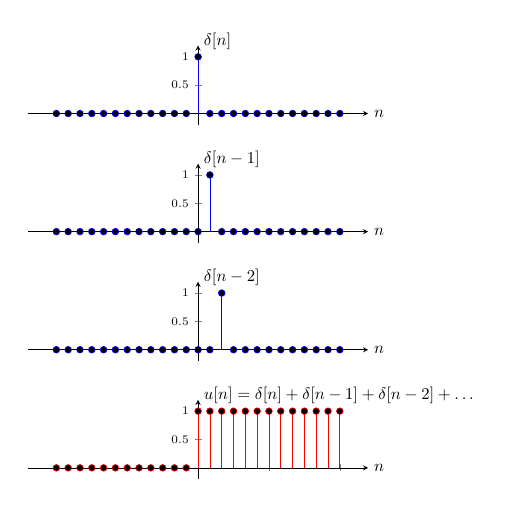
\begin{tikzpicture}[scale=0.6,
    declare function={
    unitstep(\x)= (\x>-0.1)*(1);
    impulse(\x,\nn)  = and((\nn-0.5) < \x, \x < \nn)*1;
  }
]
\begin{axis}
	[
	    scale=1,
	    axis x line=middle,
	    axis y line=middle,
	    every axis plot post/.style={mark options={fill=black}},
	    xmin=-12,
	    xmax=12,
	    xlabel={$n$},
	    ylabel={$\delta[n]$},
	    xticklabel=\empty,
	    y=1.2cm,
	    x=0.3cm,
	    ymin=-0.2,
	    ymax=1.2,
	    clip=false,
	     every axis x label/.style={at={(ticklabel* cs:1)}, anchor=west,} ,
	     every axis y label/.style={at={(ticklabel* cs:1.05)}, anchor=west,},
	]
	\addplot+[ycomb,domain=-10:10, blue] {impulse(x,0)};
\end{axis}

\pause

\begin{scope}[yshift=-2.5cm]
	\begin{axis}
	[
	    scale=1,
	    axis x line=middle,
	    axis y line=middle,
	    every axis plot post/.style={mark options={fill=black}},
	    xmin=-12,
	    xmax=12,
	    xlabel={$n$},
	    ylabel={$\delta[n-1]$},
	    xticklabel=\empty,
	    y=1.2cm,
	    x=0.3cm,
	    ymin=-0.2,
	    ymax=1.2,
	    clip=false,
	     every axis x label/.style={at={(ticklabel* cs:1)}, anchor=west,} ,
	     every axis y label/.style={at={(ticklabel* cs:1.05)}, anchor=west,},
	]
	\addplot+[ycomb,domain=-10:10, blue] {impulse(x,1)};
	\end{axis}
\end{scope}

\pause

\begin{scope}[yshift=-5cm]
	\begin{axis}
	[
	    scale=1,
	    axis x line=middle,
	    axis y line=middle,
	    every axis plot post/.style={mark options={fill=black}},
	    xmin=-12,
	    xmax=12,
	    xlabel={$n$},
	    ylabel={$\delta[n-2]$},
	    xticklabel=\empty,
	    y=1.2cm,
	    x=0.3cm,
	    ymin=-0.2,
	    ymax=1.2,
	    clip=false,
	     every axis x label/.style={at={(ticklabel* cs:1)}, anchor=west,} ,
	     every axis y label/.style={at={(ticklabel* cs:1.05)}, anchor=west,},
	]
	\addplot+[ycomb,domain=-10:10, blue] {impulse(x, 2)};
	\end{axis}
\end{scope}


\pause

\begin{scope}[yshift=-7.5cm]
	\begin{axis}
	[
	    scale=1,
	    axis x line=middle,
	    axis y line=middle,
	    every axis plot post/.style={mark options={fill=black}},
	    xmin=-12,
	    xmax=12,
	    xlabel={$n$},
	    ylabel={$u[n] = \delta[n] + \delta[n-1] + \delta[n-2] + \dots$},
	    xticklabel=\empty,
	    y=1.2cm,
	    x=0.3cm,
	    ymin=-0.2,
	    ymax=1.2,
	    clip=false,
	     every axis x label/.style={at={(ticklabel* cs:1)}, anchor=west,} ,
	     every axis y label/.style={at={(ticklabel* cs:1.05)}, anchor=west,},
	]
	\addplot+[ycomb,domain=-10:10, red] {unitstep(x)};
	\end{axis}
\end{scope}
\end{tikzpicture} 
        }
    }
\end{frame}





\begin{frame}[plain]{Continuous-Time Unit Step Function $u(t)$}
    \begin{equation}
        u(t) = \begin{cases}
                 0, & t < 0,\\
                 1, & t>0.
               \end{cases}
    \end{equation}
    \mode<beamer>
    {
        {
            \centering
            \pgfplotsset{compat=1.12}
\pgfplotsset{every tick label/.append style={font=\scriptsize}}
  \begin{tikzpicture}[scale=0.6,
  declare function={
    func(\x)= (\x<0) * (0)   +
                (\x>=0) * (1);
  }
]
  \def\omwga0{2*pi}
  \def\phase{0}
    \begin{axis}[
     clip=false,
     xmin=-12,xmax=12,
     xlabel= $t$,
     ylabel={$ u(t)$},
     ymin=-1.5,ymax=1.5,
     axis lines=middle,
     %axis x line=middle,
     %axis y line=left,
%     axis x line=middle,
     %xtick={6.28},
     %xticklabels={$T_0$},
     ytick={-1, 1},
     %yticklabels={$\small  -A$, $\small  A$},
     %xticklabel style={anchor=north west}
        x label style={at={(current axis.right of origin)},anchor=west},
        y label style={at={(current axis.above origin)}, anchor=south},
     ]
      \addplot[domain=-10:10,samples=200,red]{func(x)};


       %\draw[|-|] (axis cs: 0,1.1) -- (axis cs: 2*pi,1.1) node[midway, above] {\scriptsize $T_0=\frac{2\pi}{\omega_0}$};
       %\draw[dashed] (axis cs:2*pi, 0) -- (axis cs:2*pi, 1);
       %\node at (axis cs:0, .707) [anchor=east] {\scriptsize $A\cos\phi$  };

      % \node at (axis cs:pi, -1.2) [anchor=west] {\scriptsize $A =$ amplitude };
       %\node at (axis cs:pi, -1.4) [anchor=west] {\scriptsize $\omega_0 =$ frequency (here $\omega_0 =1$) };
       %\node at (axis cs:pi, -1.6) [anchor=west] {\scriptsize $\phi =$ phase (here $\phi =-\pi/4$) };
    \end{axis}


  \end{tikzpicture} 
        }
    }
\end{frame}



\begin{frame}[plain]{Continuous-Time Unit Impulse Function $\delta(t)$}
    \begin{columns}[t]
        \column{0.6\textwidth}
        {
            \mode<beamer>
            {
                {
                    \centering
                    \pgfplotsset{compat=1.12}
\pgfplotsset{every tick label/.append style={font=\scriptsize}}
  \begin{tikzpicture}[
  declare function={
    func(\x)= (\x<0) * (0)   +
    			and(0 < \x, \x < 1)*(\x/1) +
                (\x>= 1) * (1);
    func1(\x)= (\x<0) * (0)   +
    			and(0 < \x, \x < 1)*(1) +
                (\x>= 1) * (0);
  }
]
\begin{axis}[
		 clip=false,
        scale=0.6,
		 xmin=-5,xmax=5,
		 xlabel= $t$,
		 ylabel={$ u_\Delta(t)$},
		 ymin=-0.2,ymax=1.2,
		 axis lines=middle,
		 x = 1cm,
		 y = 2cm,
		 xticklabels=\empty,
        x label style={at={(current axis.right of origin)},anchor=west},
        y label style={at={(current axis.above origin)}, anchor=south},
	 ]
	 \addplot[domain=-5:5,samples=200,red]{func(x)};

	\draw[dashed] (axis cs:1, 1) -- (1,0) node [anchor=north] {$\Delta$};
	\node at (axis cs:6, 0.5) [anchor=west] {$u_\Delta(t) \rightarrow u(t) \text{ as } \Delta \rightarrow 0. $};
\end{axis}

\pause
\begin{axis}[
		yshift=-4.25cm,
        scale=0.6,
		 clip=false,
		 xmin=-5,xmax=5,
		 xlabel= $t$,
		 ylabel={$ \delta_\Delta(t)$},
		 ymin=-0.2,ymax=1.2,
		 axis lines=middle,
		 x = 1cm,
		 y = 2cm,
		 ytick={1},
		 yticklabels={$\dfrac{1}{\Delta}$},
		 xticklabels=\empty,
        x label style={at={(current axis.right of origin)},anchor=west},
        y label style={at={(current axis.above origin)}, anchor=south},
	 ]
	 \addplot[domain=-5:5,samples=200,red]{func1(x)};

	\path (1,0) node [anchor=north] {$\Delta$};
	\node at (axis cs:6, 0.5) [anchor=west] {$\delta_\Delta(t) \rightarrow \delta(t) \text{ as } \Delta \rightarrow 0. $};
	\node at (axis cs:6, 0.3) [anchor=west] {area = 1};	
	\draw [draw=none, pattern=north west lines, pattern color=red!80!blue!30] (axis cs:0,0) rectangle (1, 1);
\end{axis}
\pause
\begin{axis}[
		yshift=-8.5cm,
        scale=0.6,
		 clip=false,
		 xmin=-5,xmax=5,
		 xlabel= $t$,
		 ylabel={$ \delta(t)$},
		 ymin=-0.2,ymax=1.2,
		 axis lines=middle,
		 x = 1cm,
		 y = 2cm,
		 ytick={1},
		 yticklabels={$1$},
		 xticklabels=\empty,
        x label style={at={(current axis.right of origin)},anchor=west},
        y label style={at={(current axis.above origin)}, anchor=south},
	 ]

	\draw[-latex, red, thick] (axis cs:0,0) -- (axis cs:0,1);
	\node at (axis cs:6, 0.5) [anchor=west] {height = $\infty$, width = 0, area = 1};

\end{axis}

  \end{tikzpicture} 
                }
            }
        }
        \pause
        \column{0.4\textwidth}
        {
            \begin{equation}
                \delta(t) = \frac{du(t)}{dt}.
            \end{equation}
            \mode<beamer>
            {
                {
                    \centering
                    \pgfplotsset{compat=1.12}
\pgfplotsset{every tick label/.append style={font=\scriptsize}}
  \begin{tikzpicture}[scale=0.6,
  declare function={
    func(\x)= (\x<0) * (0)   +
                (\x>=0) * (1);
  }
]
  \def\omwga0{2*pi}
  \def\phase{0}
    \begin{axis}[
     clip=false,
     xmin=-12,xmax=12,
     xlabel= $t$,
     ylabel={$ \delta(t)$},
     ymin=-1.5,ymax=1.5,
     axis lines=middle,
     %axis x line=middle,
     %axis y line=left,
%     axis x line=middle,
     xtick={-5, 0, 5},
     xticklabels={-5, 0, 5},
     ytick={-1, 0, 1},
     %yticklabels={$\small  -A$, $\small  A$},
     %xticklabel style={anchor=north west}
        x label style={at={(current axis.right of origin)},anchor=west},
        y label style={at={(current axis.above origin)}, anchor=south},
     ]
     %\addplot[domain=-10:10,samples=200,red]{func(x)};
      \draw[-latex, thick, red] (axis cs:0,0) -- (axis cs:0,1);
      \node at (axis cs:0,-.15) [anchor= east] {\scriptsize 0};


       %\draw[|-|] (axis cs: 0,1.1) -- (axis cs: 2*pi,1.1) node[midway, above] {\scriptsize $T_0=\frac{2\pi}{\omega_0}$};
       %\draw[dashed] (axis cs:2*pi, 0) -- (axis cs:2*pi, 1);
       %\node at (axis cs:0, .707) [anchor=east] {\scriptsize $A\cos\phi$  };

      % \node at (axis cs:pi, -1.2) [anchor=west] {\scriptsize $A =$ amplitude };
       %\node at (axis cs:pi, -1.4) [anchor=west] {\scriptsize $\omega_0 =$ frequency (here $\omega_0 =1$) };
       %\node at (axis cs:pi, -1.6) [anchor=west] {\scriptsize $\phi =$ phase (here $\phi =-\pi/4$) };
    \end{axis}


  \end{tikzpicture} 
                }
                \pause
                \begin{equation*}
                    x(t)\delta(t) = x(0)\delta(t)
                \end{equation*}
                \begin{equation*}
                    x(t)\delta(t -t_0) = x(t_0)\delta(t-t_0)
                \end{equation*}
                
            }
        }
    \end{columns}




\end{frame}

\begin{frame}[plain]{CT Unit Step Function and Unit Impulse Function}
    \begin{equation}
        u(t) = \int_{-\infty}^{t}\delta(\tau)d\tau.
    \end{equation}
        \mode<beamer>
        {
            {
                \centering
                \begin{tikzpicture}[
  declare function={
    unitstep(\x)= (\x>-0.1)*(1);
  },
    declare function={
    unitstepdelayed(\x)= (\x>0.1)*(1);
  },
    declare function={
    impulse(\x)= and(\x>-0.1, \x<0.1)*(1);
  }
]
\begin{axis}
[
        scale=0.6,
    axis x line=middle,
    axis y line=middle,
    every axis plot post/.style={mark options={fill=black}},
    xmin=-12,
    xmax=12,
    xlabel={$\tau$},
    ylabel={$$},
    y=1.2cm,
    x=0.3cm,
    ymin=-0.2,
    ymax=1.5,
   ytick={1},
   yticklabels={1},
   xticklabels=\empty,
    clip=false,
        x label style={at={(current axis.right of origin)},anchor=west},
        y label style={at={(current axis.above origin)}, anchor=south},
]
\draw[draw=none, pattern=north west lines, pattern color=red!80!blue!30] (axis cs:-12, 1.2) rectangle (axis cs:-3, 0);
%\addplot+[ycomb,domain=-10:10, blue] {impulse(x)};
\draw[red, dashed, thick] (axis cs:-12, 1.2) -| (axis cs:-3, 0) node [anchor=north, yshift=-3pt] {$t$};
\draw[blue, thick, -latex] (axis cs: 0, 0) -| (axis cs:0, 1);
\node at (axis cs: 0, 0)  [anchor=north, yshift=-3pt] {0};
\node at (axis cs:4, 1)  [] {$t<0$};
\end{axis}

\pause

\begin{scope}[yshift=-3cm]
	\begin{axis}
[
        scale=0.6,
    axis x line=middle,
    axis y line=middle,
    every axis plot post/.style={mark options={fill=black}},
    xmin=-12,
    xmax=12,
    xlabel={$\tau$},
    ylabel={$$},
    y=1.2cm,
    x=0.3cm,
    ymin=-0.2,
    ymax=1.5,
   ytick={1},
   yticklabels={1},
   xticklabels=\empty,
    clip=false,
        x label style={at={(current axis.right of origin)},anchor=west},
        y label style={at={(current axis.above origin)}, anchor=south},
]
%\addplot+[ycomb,blue] table [x={n}, y={xn}] {step.dat};
\draw[draw=none, pattern=north west lines, pattern color=red!80!blue!30] (axis cs:-12, 1.2) rectangle (axis cs:3, 0);
%\addplot+[ycomb,domain=-10:10, blue] {impulse(x)};
\draw[red, dashed, thick] (axis cs:-12, 1.2) -| (axis cs:3, 0) node [anchor=north, yshift=-3pt] {$t$};
\draw[blue, thick, -latex] (axis cs: 0, 0) -| (axis cs:0, 1);
\node at (axis cs: 0, 0)  [anchor=north, yshift=-3pt] {0};
\node at (axis cs:4, 1)  [] {$t>0$};
\end{axis}
\end{scope}

\end{tikzpicture} 
            }
        }
\end{frame}



\subsection{Signal Energy and Power}

\begin{frame}[allowframebreaks]{Energy}
    The total energy over a time interval $t_1 \leq t \leq t_2$ in a continuous-time signal $x(t)$ is
    \begin{equation*}
        \int_{t_1}^{t_2}|x(t)|^2dt
    \end{equation*}
    The total energy over a time interval $n_1 \leq n \leq n_2$ in a discrete-time signal $x[n]$ is
    \begin{equation*}
        \sum_{n= n_1}^{n_2}|x[n]|^2dt
    \end{equation*}
    Total energy  over an infinite interval in a CT signal:
    \begin{equation}
        E_\infty \triangleq \lim_{T \rightarrow \infty} \int_{-T}^{T}|x(t)|^2dt =  \int_{-\infty}^{+\infty}|x(t)|^2dt.
    \end{equation}
    Total energy  over an infinite interval in a DT signal:
    \begin{equation}
      E_\infty \triangleq \lim_{N \rightarrow \infty} \sum_{n = -N}^{+N}|x[n]|^2 =  \sum_{n=-\infty}^{+\infty}|x[n]|^2.
    \end{equation}
    Note that this integral and may not converge for some signals. Such signals have infinite energy, while signals with $E_\infty < \infty$ have finite energy.
\end{frame}


\begin{frame}{Power}

    Time-averaged power over an infinite interval in a CT signal:
    \begin{equation}
        P_\infty \triangleq \lim_{T \rightarrow \infty} \frac{1}{2T}\int_{-T}^{T}|x(t)|^2dt.
    \end{equation}
    Total energy in a DT signal:
    \begin{equation}
      P_\infty \triangleq \lim_{N \rightarrow \infty} \frac{1}{2N+1}\sum_{n = -N}^{+N}|x[n]|^2.
    \end{equation}
    With these definitions, we can identify three important classes of signals:
    \begin{enumerate}
        \item Energy signals: Signals with finite total energy $E_\infty < \infty$. These have zero average power.
        \item Power signals: Signals with finite average power $0 < P_\infty < \infty$. As $P_\infty > 0$, $E_\infty = \infty$.
        \item Signals with neither $E_\infty$ nor $P_\infty$ are finite.
    \end{enumerate}
\end{frame} 